\documentclass[a4paper,12pt]{article} % тип документа

% Поля страниц
\usepackage[left=2.5cm,right=2.5cm,
    top=2cm,bottom=2cm,bindingoffset=0cm]{geometry}
    
%Пакет для таблиц   
\usepackage{multirow} 
    
%Отступ после заголовка    
\usepackage{indentfirst}

% Рисунки
\usepackage{floatrow,graphicx,calc}
\usepackage{wrapfig}

%%% Работа с картинками
\usepackage{graphicx}  % Для вставки рисунков
\graphicspath{{images/}}  % папки с картинками
\setlength\fboxsep{3pt} % Отступ рамки \fbox{} от рисунка
\setlength\fboxrule{1pt} % Толщина линий рамки \fbox{}
\usepackage{wrapfig} % Обтекание рисунков и таблиц текстом

% Создаём новый разделитель
\DeclareFloatSeparators{mysep}{\hspace{1cm}}

% Ссылки?
\usepackage{hyperref}
\usepackage[rgb]{xcolor}
\hypersetup{				% Гиперссылки
    colorlinks=true,       	% false: ссылки в рамках
	urlcolor=blue          % на URL
}


%  Русский язык
\usepackage[T2A]{fontenc}			% кодировка
\usepackage[utf8]{inputenc}			% кодировка исходного текста
\usepackage[english,russian]{babel}	% локализация и переносы

% Математика
\usepackage{amsmath,amsfonts,amssymb,amsthm,mathtools}

%%% Дополнительная работа с математикой
\usepackage{amsmath,amsfonts,amssymb,amsthm,mathtools} % AMS
\usepackage{icomma} % "Умная" запятая: $0,2$ --- число, $0, 2$ --- перечисление

% Что-то 
\usepackage{wasysym}


\begin{document}
\begin{center}
	\footnotesize{ФЕДЕРАЛЬНОЕ ГОСУДАРСТВЕННОЕ АВТОНОМНОЕ ОБРАЗОВАТЕЛЬНОЕ 			УЧРЕЖДЕНИЕ ВЫСШЕГО ОБРАЗОВАНИЯ}\\
	\footnotesize{МОСКОВСКИЙ ФИЗИКО-ТЕХНИЧЕСКИЙ ИНСТИТУТ\\(НАЦИОНАЛЬНЫЙ 			ИССЛЕДОВАТЕЛЬСКИЙ ИНСТИТУТ)}\\
	\footnotesize{ФИЗТЕХ-ШКОЛА ФИЗИКИ И ИССЛЕДОВАНИЙ им. ЛАНДАУ\\}
	\hfill \break
	\hfill \break
	\hfill \break
	\hfill \break
\end{center}

\begin{center}   
    \hfill \break
	\hfill \break
	\hfill \break
	\hfill \break    \hfill \break
	\hfill \break
	\hfill \break
	\hfill \break
    \hfill \break
    \hfill \break
	\hfill \break
	\large{Лабораторная работа № 2.2.1\\\textbf{Исследование взаимной диффузии газов}}\\
	\begin{flushright}
		Плотникова Анастасия Александровна\\
		Группа Б02-406
	\end{flushright}
	\hfill \break
	\hfill \break
	\hfill \break
\end{center}
\hfill \break
\hfill \break
\hfill \break
\hfill \break
\hfill \break
\hfill \break
\hfill \break
\hfill \break
\hfill \break
\hfill \break
\hfill \break
\hfill \break
\hfill \break
\begin{center}
	Долгопрудный, 2025 г.
\end{center}
\thispagestyle{empty}
\newpage
	\textbf{Цель работы:}\\ 
  1) регистрация зависимости концентрации гелия в воздухе от времени с помощью датчиков теплопроводности при разных начальных давлениях смеси газов;\\ 
  2) определение коэффициента диффузии по результатам измерений.
	\hfill \break
	
	\textbf{В работе используются:}\\ 
  измерительная установка;\\ 
  форвакуумный насос ADVAVAC-2;\\ 
  баллон с гелием при высоком давлении;\\ 
  манометр;\\ 
  датчики теплопроводности; \\
  источник питания;\\ 
  магазин сопротивлений;\\ 
  вольтметр B7-78: 
  \par диапазон: 100 мВ, 
  \par погрешность в данном диапазоне: $\pm (0.0035 \% \text{ изм.} + 0.0005 \% \text{ диап.})$.
	\hfill \break

\section*{Теоретическая справка}

\textit{Диффузией} называется самопроизвольное перемешивание молекул, происходящее вследствие их хаотичного теплового движения.

При перемешивании молекул разного сорта говорят о взаимной (или концентрационной) диффузии. 

Для наблюдения взаимной диффузии необходимо равенство давлений во всей системе (в противном случае возникнет гораздо более быстрое макроскопическое течение газа как сплошной среды).

\medskip

Пусть система состоит из двух компонетов a и b. 
Тогда плотность потока вещества любого компонента в результате взаимной диффузии определяется законом Фика. 

\begin{equation}
  j_a = - D_{ab} \frac{\delta n_a}{\delta x}, \quad j_b = - D_{ba} \frac{\delta n_b}{\delta x}
\end{equation}
где $D_{ab} = D_{ba} = D$ — коэффициент взаимной диффузии компонентов,\\ а $j_{a,b}$ — плотности потока частиц соответствующего сорта.

Исследуется диффузия примеси гелия на фоне воздуха. В условиях опыта $n_{\text{возд}} \gg n_{He}$, относительное изменение концентрации воздуха в результате взаимной диффузии мало. С достаточной точностью будем описывать только диффузию гелия на фоне воздуха. Далее $n = n_{He}$.

\section*{Экспериментальная установка}

Схема установки изображена на рисунке (\ref{fig:dr1}). 

\begin{figure}[h]
  \centering
  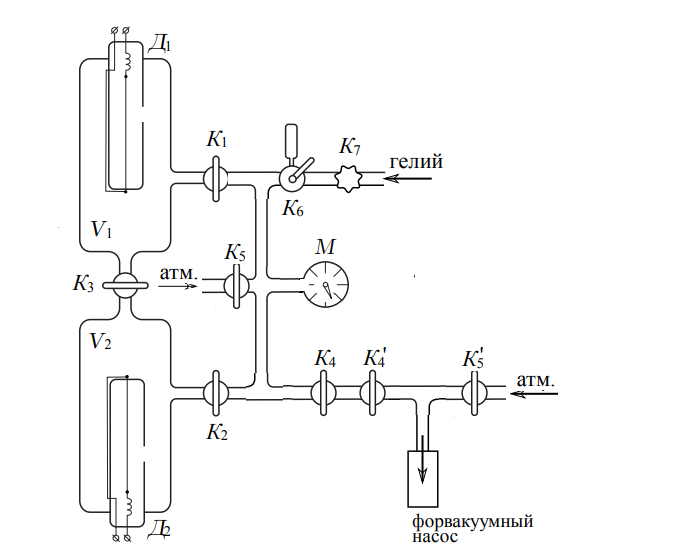
\includegraphics[scale = 0.6]{drawing1.jpg}
  \caption{Установка для исследования взаимной диффузии газов}
  \label{fig:dr1}
\end{figure}

Два сосуда с объёмами $V_1$ и $V_2$ соединены трубкой длины $l$ и сечения $S$. Сосуды заполнены смесью двух газов при одинаковом давлении, но с различной концентрацией компонентов. Вследствие взаимной диффузии концентрации каждого из компонентов в обоих сосудах с течением времени выравниваются.

Если бы концентрации в сосудах $V_1$ и $V_2$ поддерживались постоянными и равными $n_1$ и $n_2$, то в трубке установился бы стационарный поток частиц $J = - DS \frac{\delta n}{\delta x}$, одинаковый в каждом сечении трубки. Следовательно, $n(x)$ была бы линейной функцией координаты и $\frac{dn}{dx} = \frac{\Delta n}{l}$, где $l$ — длина трубки. 

\begin{equation}
  J = - DS \frac{n_1 - n_2}{l} 
\end{equation}
\begin{equation}
  V_1 \Delta n_1 = - V_2 \Delta n_2 = J \Delta t = - DS \frac{n_1 - n_2}{l} \Delta t
\end{equation}
\begin{equation}
  V_1 \frac{dn_1}{dt} = - DS \frac{n_1 - n_2}{l}, \quad V_2 \frac{dn_2}{dt} = DS \frac{n_1 - n_2}{l}
\end{equation}
\begin{equation}
  \frac{dn_1}{dt} - \frac{dn_2}{dt} = - \frac{n_1 - n_2}l DS \left( \frac1{V_1} + \frac1{V_2} \right)
\end{equation}
Введем новую переменную $\Delta n = n_1 - n_2$:
\begin{equation}
  d(\Delta n) = d(n_1 - n_2) = - \frac{n_1 - n_2}l DS \left( \frac1{V_1} + \frac1{V_2} \right) = - \frac{\Delta n}l DS \left( \frac1{V_1} + \frac1{V_2} \right)
\end{equation}
Проинтегрируем:
\begin{equation}
  \Delta n = \Delta n_0 \exp \left( \frac{l}{DS} \left( \frac{1}{V_1} + \frac{1}{V_2} \right) \right) = \Delta n_0 e^{-t/\tau},
  \label{exp}
\end{equation}
где $\Delta n_0$ - разность концентраций примеси в начльный момент времени, а \( \tau = \frac{V_1 V_2}{V_1 + V_2} \frac {l}{SD} \).

Так, разность концентраций убывает по экспоненциальному закону. Характерное время $\tau$ определяется геометрическими параметрами установки и величиной коэффициента диффузии.

Модель квазистационарного течения применима, если время $\tau$ много больше характерного времени диффузии одной частицы вдоль трубки длиной $l$ (\( t_{\text{diff}} \sim \frac{l^2}{D} \ll \tau \)).

\medskip

Для измерения концентраций применяются датчики теплопроводности $D_1$ и $D_2$ и используется зависимость теплопроводности газовой смеси от её состава. 

Тонкая проволока радиуса $r$, протянутая вдоль оси цилиндра радиуса $R$, нагревается током. Тепло от проволоки к стенке цилиндра передаётся главным образом вспледствие теплопроводности газа, находящегося внутри цилиндра. 

Плотность теплового потока в условиях цилиндрической симметрии:
\begin{equation}
  q = - \kappa \frac{d T}{d r}
\end{equation}

Количество тепла переданного стенке цилиндра в единицу времени:
\begin{equation}
  Q = q \cdot S = q \cdot 2 \pi r L = 2 \pi r L (- \kappa \frac{d T}{d r})
\end{equation}

Пренебрежем потерями через торцы и теплопередачей излучением. Тогда тепловой поток $Q$ равен теплу, выделяемому в нити. Значит, $Q$ не зависит от $r$.
\begin{equation}
  - \frac{Q}{2 \pi L \kappa} \cdot \frac{d r}{r} = d T
\end{equation}

\begin{equation}
  - \Delta T = T_1 - T_2 = \frac{Q}{2 \pi L \kappa} \text{ln} \frac{r_2}{r_1}
\end{equation}

\begin{equation}
Q = \kappa \frac{2\pi L}{ln (R/r)}(T_1-T_2)
\end{equation}
где $\kappa$ — теплопроводность, \\
$L$ - длина нити, \\
$T_1$ — температура проволоки, \\
$T_2$ — температура стенки. 

При $Q = \text{const}$ температура проволоки и её сопротивление определяются теплопроводностью газа и, следовательно, его составом. Для измерения разности концентраций газов используется мостовая схема, изображенная на рисунке (\ref{fig:bridge}).

Мост балансируется при заполнении сосудов одной и той же смесью.

\begin{figure}[h]
  \centering
  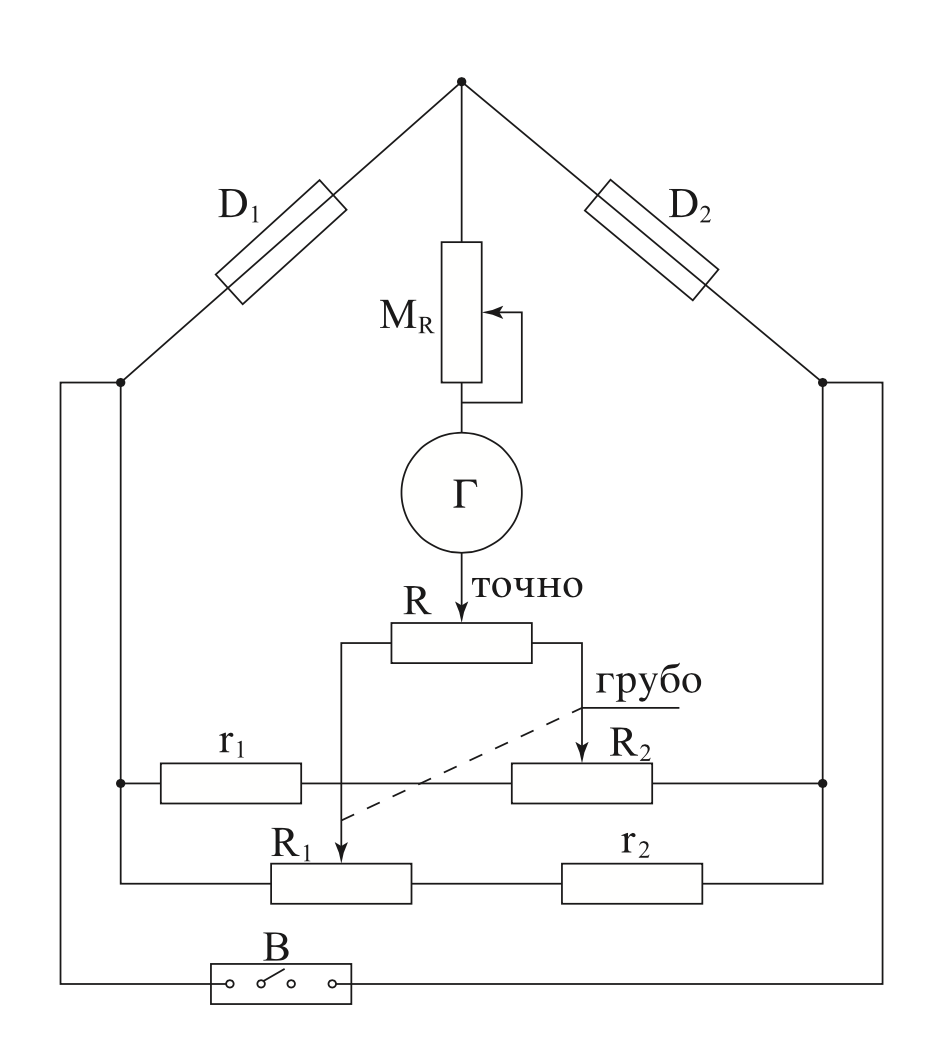
\includegraphics[scale = 0.40]{bridge.png}
  \caption{Мостовая схема с датчиками теплопроводности для измерения разности концентраций газов}
  \label{fig:bridge}
\end{figure}

\noindent $D_1$, $D_2$ — датчики теплопроводности, \\
$R$ — для балансировки (точно), \\
$R_1$, $R_2$ — для балансировки (грубо).

В процессе диффузии показания гальванометра убывают по экспоненциальному закону:
\begin{equation}
  U = U_0 e^{-t/\tau}
\end{equation}

По тому же закону изменяется разность концентраций. Измерив зависимость $U(t)$ получим характерное время процесса, откуда определим коэффициент диффузии.

\section*{Ход работы}

\begin{enumerate}
  \item Ознакомимся с конструкцией нашей установки. По дополнительным описаниям, расположенным на столах, изучим:
  \begin{enumerate}
    \item схему подачи воздуха и гелия и схему откачки нашей установки;
    \item особенности измерительных приборов, используемых в нашей установке (манометр, вольтметр); вычислим цену деления шкалы манометра в торрах.

    $p_{\text{атм}} = (748.6 \pm 0.3)$ торр. \\
    $\Delta p_{\text{max}} = (100.5 \pm 0.5)$ дел. — показания вакууметра при полной откачке установки.

    Приравняв $p_{\text{атм}}$ и $\Delta p_{\text{max}}$, получим, что одно деление вакууметра соответствует $(7.45 \pm 0.04)$ торр.
    
    \item включим компьютер и запустим расчётную программу, ознакомимся с краткой инструкцией её использования.
    
  \end{enumerate}

  Также изучим параметры установки: \\
  $V_1 = V_2 = V = (1200 \pm 30) \, \text{см}^3$ \\
  $L/S = (5.5 \pm 0.5) \, \text{см}^{-1}$ 
  
  \item Подготовим установку к работе:
  \begin{enumerate}
    \item включим питание датчиков, вольтметра и измерительного моста;
    \item убедимся, что кран подачи гелия $K_7$ и все краны на атмосферу $K_5,\, K_5'$ плотно закрыты, и в установке нет запертых объёмов;
    \item включим форвакуумный насос, откачаем сначала сам насос, затем откроем $K_4$ и будем откачивать установку примерно 2-3 минуты до момента, когда показания вакууметра достигнут максимума;
    \item после окончания откачки закроем $K_4$, выключим насос и откроем атмосферный кран.
  \end{enumerate}
  
  \item Рассчитаем, какой отметке вакууметра соответствует рабочее давление $P_\text{раб} = \alpha (P_0 - P)$. Здесь $P$, $P_0$ — значение показаний вакууметра в момент измерений и при максимальном достигаемом вакууме, а $\alpha = (7.45 \pm 0.04) \frac{\text{торр}}{\text{дел.}}$ — коэффициент пересчёта.
  
  Обозначив показания вакууметра за $\Delta P$, получим:
  
  \begin{table}[h!]
    \begin{tabular}{|l|c|c|c|c|c|c|}
      \hline
      № & 1 & 2 & 3 & 4 & 5 & $\sigma$ \\
      \hline 
      $P$, дел. & 95.0 & 91.0 & 85.0 & 79.0 & 73.5& 0,5 \\ 
      $P_{\text{раб}}$, торр & 41 & 71 & 116 & 160 & 201 & 5\\
      \hline    
    \end{tabular}
    \caption{Рабочие давления в диапазоне 40-200 торр}
    \label{tab:P}
  \end{table}
  
  \begin{equation}
    \varepsilon(P_\text{раб}) = \varepsilon_{\text{вак}}^0 + \varepsilon_{\text{вак}} + \varepsilon_{\alpha} = \frac{d P_0}{P_0} + \frac{d P}{P} + \frac{d \alpha}{\alpha} = \frac{0.5}{100.5} + \frac{0.5}{73.5} + \frac{0.04}{7.45} = 0.017 
  \end{equation}

  \begin{equation}
    d(P_\text{раб}) = P_\text{раб} \cdot \varepsilon(P_\text{раб}) 
  \end{equation}
  
  
  Сбалансируем измерительный мост при предполагаемом рабочем давлении:
  \begin{enumerate}
    \item напустим в установку воздух до давления $P_\text{раб}$;
    \item изолируем рабочие объёмы, закрыв краны $K_1$, $K_2$;
    \item сбалансируем измерительный мост так, чтобы показания вольтметра флуктуировали около нулевого значения, в мВ сохраняя два-три нуля после запятой.
  \end{enumerate}
  
  \item Приготовим рабочие смеси для проведения измерений:
  \begin{enumerate}
    \item откачаем всю установку до максимальных показаний вакууметра;
    \item изолируем объём $V_2$, закрыв краны $K_2$ и $K_3$, выключим насос;
    \item откроем кран подачи гелия $K_7$, с помощью дозатора напустим в установку гелий до давления $P_{He} = 0.2 P_\text{раб}$;
    \item перекроем подачу гелия и откачаем гелий из всех патрубков;
    \item присоединим объём $V_2$ к установке и заполним её воздухом до давления $1.75 P_\text{раб}$;
    \item откроем $K_1$ и $K_2$, уравняем давления в сосудах $V_1$ и $V_2$ за счет добавления воздуха в верхний сосуд;
    \item запишем точное значение установившегося рабочего давления $P_\text{раб}$.
  \end{enumerate}
  Изолируем объемы. Так, в нижнем сосуде (2) остался чистый воздух, а в верхнем (1) — смесь гелия с воздухом.
  
  \item Запустим процесс диффузии после открытия крана $K_3$. Откроем $K_3$ и измерим, как меняются показания вольтметра с течением времени $U(t)$. 
  
  \item Повторим измерения при различных значениях рабочего давления в диапазоне $40-200$ торр. Программа, которая снимает данные, фиксирует достаточно много точек. Ограничимся их выборкой:

  \begin{table}[h!]
    \centering
    \begin{tabular}{|c|c|c|c|c|c|c|c|c|c|}
      \hline
      \multicolumn{2}{|c|}{41 торр} & \multicolumn{2}{c|}{71 торр} & \multicolumn{2}{c|}{116 торр} & \multicolumn{2}{c|}{160 торр} & \multicolumn{2}{c|}{201 торр} \\ \hline
      $t$, с & $U$, мВ & $t$, с & $U$, мВ & $t$, с & $U$, мВ & $t$, с & $U$, мВ & $t$, с & $U$, мВ \\ 
      \hline 
      0      & 18,7979 & 0     & 19,9714 & 0        & 19,9101 & 0      & 20,7675 & 0 & 19,6310 \\
      30,890 & 17,1361 & 60,931 & 17,8623 & 120,906 & 17,3759 & 120,849 & 18,8170 & 120,197 & 18,1859 \\
      60,891 & 15,6902 & 120,930 & 16,1379 & 240,906 & 15,3942 & 240,850 & 17,2460 & 240,197 & 16,9559 \\
      90,890 & 14,4141 & 90,930 & 16,9715 & 360,907 & 13,6841 & 360,849 & 15,8147 & 360,197 & 15,8181 \\
      120,890 & 13,1600 & 180,931 & 14,6330 & 480,906 & 12,1794 & 480,850 & 14,5285 & 480,197 & 14,7564 \\
      150,890 & 12,0771 & 150,930 & 15,3691 & 600,906 & 10,8797 & 600,849 & 13,3443 & 600,197 & 13,7834 \\
      180,890 & 11,0807 & 240,931 & 13,2948 & 719,906 & 9,7007 & 720,849 & 12,2722 & 720,197 & 12,8880 \\
      \hline  
    \end{tabular}
    \caption{Примеры показаний вольтметра при каждом из рабочих давлений}
    \label{tab:example}
  \end{table}
  
  Полученная зависимость $U(t)$ представлена на графике (\ref{fig:raw}):
  
  \begin{figure}[h!]
    \centering
    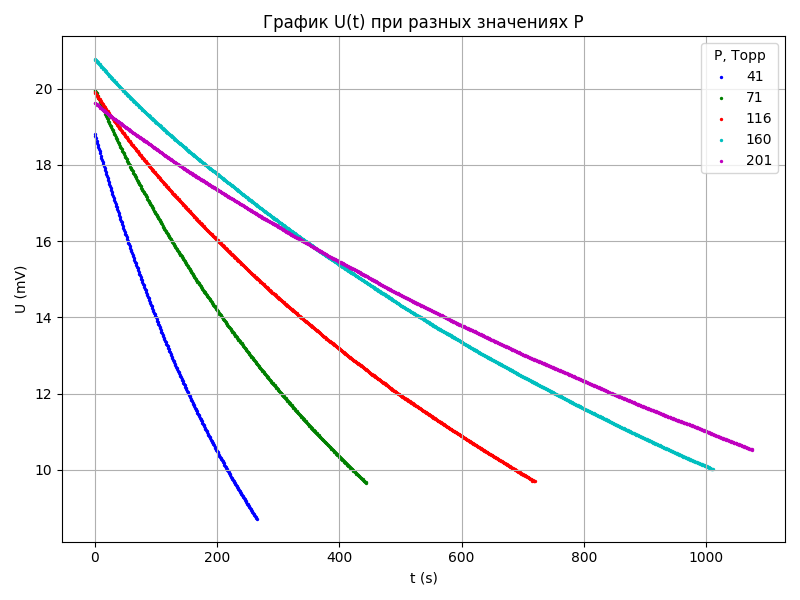
\includegraphics[scale = 0.75]{graph_raw.png}
    \caption{Зависимость $U(t)$ при разных значениях давлений $P$}
    \label{fig:raw}
  \end{figure}
  \item (Дополнительно) Коэффициент диффузии примеси воздуха в гелии не измеряем.
  
  \item Убедимся, что процесс диффузии подчиняется закону (\ref{exp}). Для этого построим графики зависимости $U(t)$ в логарифмическом масштабе. 
  
  Зависимость $\text{ln} (U / U_0)$, где $U_0$ — показания вольтметра в момент начала отсчета, представлена на графике (\ref{fig:ln}).

  \begin{figure}
    \centering
    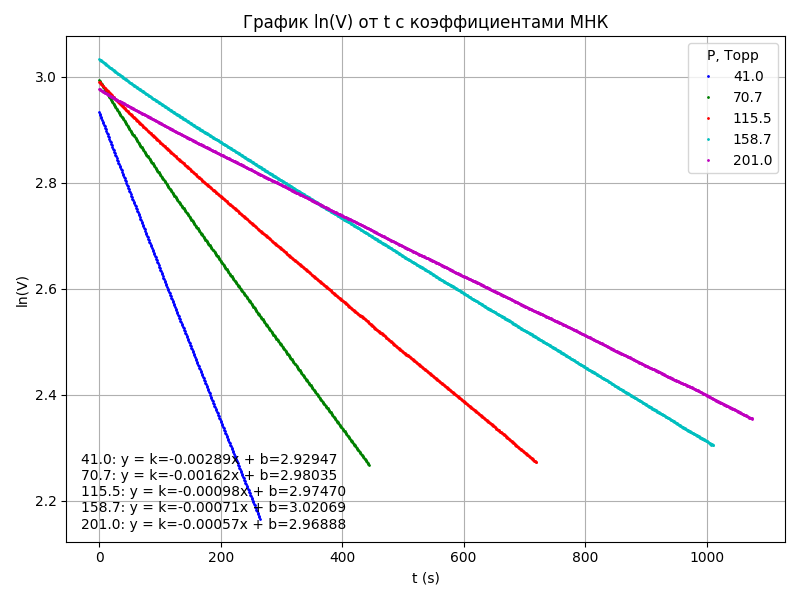
\includegraphics[scale = 0.75]{graph_ln.png}
    \caption{Зависимость $\text{ln} (U / U_0)$ от $t$ при разных значениях давлений $P$}
    \label{fig:ln}
  \end{figure}

  Рассчитаем коэффициенты взаимной диффузии при выбранных рабочих давлениях по формуле $D = -\frac{kVL}{2S}$, где $k$ — коэффициент наклона прямой, апроксимирующей логарифмическую зависимость согласно МНК. Их погрешность составит:
  \begin{equation}
    \sigma_D = D \sqrt{\left( \frac{\sigma_V}{V} \right) ^ 2 + \left( \frac{\sigma_k}{k} \right) ^ 2 + \left( \frac{\sigma_{L/S}}{L/S} \right) ^ 2}
  \end{equation}

  Коэффициенты наклона и взаимной диффузии представлены в таблице (\ref{tab:k}).
  
  \begin{table}[h!]
    \centering
    \begin{tabular}{|c|c|c|c|c|} 
      \hline
      $P$, торр & $k, \, 10^{-3}$ c$^{-1}$ & $\varepsilon_k, \, \%$ & $D$, см$^2$/c & $1/P$, торр$^{-1}$ \\
      \hline 
      41  & $-(2.894 \pm 0.001)$    & 0.04  & 9.6 $\pm$ 0.9   & 0.024 $\pm$ 0.003  \\
      71  & $-(1.619 \pm 0.002)$    & 0.10  & 5.3 $\pm$ 0.5   & 0.014 $\pm$ 0.001 \\
      116 & $-(0.983 \pm 0.001)$    & 0.08  & 3.2 $\pm$ 0.3   & 0.0086 $\pm$ 0.0004\\
      160 & $-(0.7123 \pm 0.0003)$  & 0.04  & 2.4 $\pm$ 0.2   & 0.0062 $\pm$ 0.0002 \\
      201 & $-(0.5721 \pm 0.0002)$  & 0.03  & 1.89 $\pm$ 0.18 & 0.0050 $\pm$ 0.0001 \\
      \hline
    \end{tabular}
    \caption{Значения $P, \, k, \, \varepsilon_k, \, D, \, 1/P$}
    \label{tab:k}
  \end{table}

  Рассчитаем $1/P$ и погрешность этой величины и занесём в ту же таблицу.

  \begin{equation}
    \sigma_{1/P} = \frac{\partial \left( {1}/{P} \right)}{\partial P} \cdot \sigma_P = -\frac{1}{P^2} \cdot \sigma_P
  \end{equation}
  
  \item Построим график зависимости коэффициента диффузии от обратного давления в координатах $D(1/P)$, см. рисунок (\ref{fig:D_1P}).
  
  \begin{figure}[h!]
    \centering
    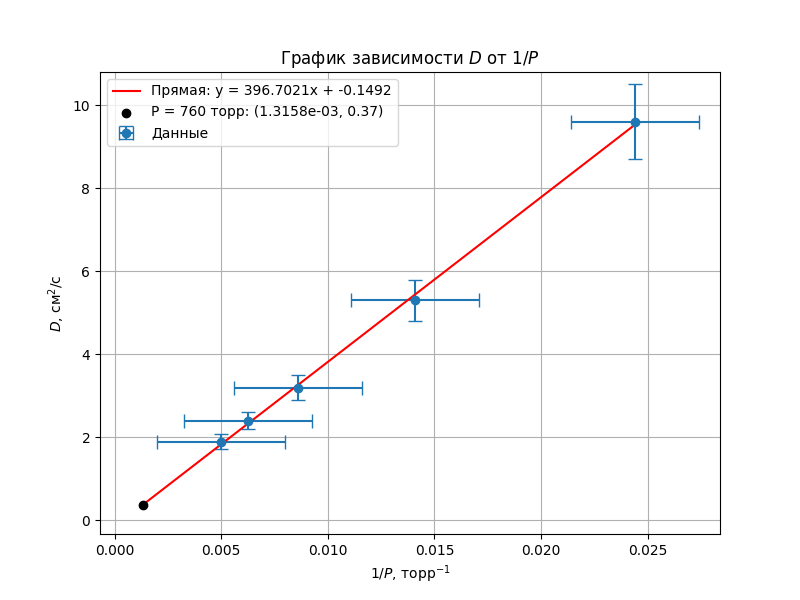
\includegraphics[scale = 0.75]{graph_D_1P.png}
    \caption{Зависимость $D(1/P)$}
    \label{fig:D_1P}
  \end{figure}

  Найдем угловой коэффициент $k' = \frac{d(D)}{d(1/P)}$ графика (\ref{fig:D_1P}) с помощью метода наименьших квадратов.

  \begin{equation}
    k' = \frac{d(D)}{d(1/P)} = \frac{\langle \frac{1}{P} D \rangle - \langle \frac{1}{P} \rangle \langle D \rangle}{\langle \frac{1}{P^2} \rangle - \langle \frac{1}{P} \rangle ^2} = 396.70 \, \text{см}^2 / \text{c}
    \label{k1}
  \end{equation}

  \begin{equation}
    \label{dk1}
    dk' = \frac{1}{\sqrt{n}} \sqrt{\frac{\langle D^2 \rangle - \langle D \rangle ^2}{\langle \frac{1}{P^2} \rangle - \langle \frac{1}{P} \rangle} - k'^2} = 7.16 \, \text{см}^2 / \text{c}
  \end{equation}

  \begin{equation}
    \label{ek}
    \varepsilon_{k'_{\text{МНК}}} = \left| \frac{dk'}{k'} \right| = 0,018
  \end{equation}

  Учтем погрешность прямых измерений.

  \begin{equation}
    \varepsilon_{k'_{\text{ИЗМ}}}= \varepsilon ({d(D)}) + \varepsilon({d(1/P)}) = \sqrt{\frac{dD}{D}^2 + \frac{dP}{P^2}^2} = 0.118
  \end{equation}

  Из-за небольшого количества точек $(n = 5)$ для оценки погрешности необходимо учитывать коэффициент Стьюдента. Примем доверительный интервал 95\%, тогда согласно таблице: $t \approx 3,18$.

  Обозначим стандартное отклонение за $s$ и стандартную ошибку за $s_{k'}$. Вычислим вклад коэффициента Стьюдента в относительную погрешность $k'$.
  \begin{equation}
    \varepsilon_{k'} = \frac{t \cdot s_{k'}}{k'}, \qquad 
    s_{k'} = \frac{s}{\sqrt{\sum (1/P_i - \langle 1/P \rangle)^2}} = 
    \frac{\sqrt{\frac{\sum (D_i - k' (1/P_i))^2}{n - 2}}}{\sqrt{\sum (1/P_i - \langle 1/P \rangle)^2}}
  \end{equation}
  \begin{equation}
    \varepsilon_{k'_{\text{СТ}}} = 0.121
  \end{equation}

  Получается:
  \begin{equation}
    \varepsilon_{k'} = \sqrt{\varepsilon_{k'_{\text{МНК}}}^2 + \varepsilon_{k'_{\text{ИЗМ}}}^2 + \varepsilon_{k'_{\text{СТ}}}^2} = 0.17, \qquad d(k') = \varepsilon_{k'} \cdot k' = 67.4 \, \text{см}^2 / \text{c}
  \end{equation}
  

  \begin{equation}
    k' = (400 \pm 70) \, \text{см}^2 / \text{c} \qquad (17\%)
  \end{equation}

  Экстраполируя график к атмосферному давлению, оценим соответствующий коэффициент диффузии.

  \begin{equation}
    D_{\text{атм}} = k' (1 / P_{\text{атм}}) + b' = 0.3728 \, \text{см}^2/\text{c}
  \end{equation}
  \begin{equation}
    D_{\text{атм}} = (3.7 \pm 0.6) \cdot 10^{-1} \, \text{см}^2/\text{c}
    \label{Datm}
  \end{equation}
  
  \item (Дополнительно) Коэффициенты диффузии примеси гелия в воздухе $D_{He-\text{возд}}$ и примеси воздуха в гелии $D_{\text{возд}-He}$ не сравниваем.
  
  \item Оценим длину свободного пробега атомов гелия в воздухе $\lambda_{He}$ в условиях эксперимента. 
  \begin{equation}
    \lambda = 3D \sqrt{\frac{\pi \mu }{8RT}} = 62.29 \, \text{нм}
  \end{equation}
  \begin{equation}
  \delta \lambda = \left| -\frac{3D \sqrt{\frac{\pi \mu}{8R}}}{2T^{3/2}} \right| \delta T = 0.21 \, \text{нм}
  \end{equation}  
  \begin{equation}
    \lambda = (6.23 \pm 0.02) \cdot 10^{-8} \, \text{м}
  \end{equation}

  Оценим эффективное сечение столкновений атомов гелия с молекулами воздуха $\sigma_{He-\text{возд}}$.
  \begin{equation}
  \sigma = \frac{1}{\lambda n} = \frac{kT}{\lambda P} = 6.66 \cdot 10^{-19} \, \text{м}^2
  \end{equation}
  \begin{equation}
  \delta \sigma = \sqrt{\left( \frac{k}{\lambda P} \delta T \right)^2 + \left( -\frac{kT}{\lambda P^2} \delta P \right)^2} = 4.50 \cdot 10^{-21} \, \text{м}^2
  \end{equation}
  \begin{equation}
    \sigma = (6.66 \pm 0.05) \cdot 10^{-19} \, \text{м}^2
  \end{equation}

  Везде принимаем $T = (300 \pm 2)$ К, $P = (99800 \pm 40) $ Па. Табличные константы берем с такой точностью, чтобы пренебречь их погрешностью в расчётах.

\end{enumerate}

\section*{Вывод}

Все цели работы были достигнуты.

\begin{enumerate}
  \item Изучена зависимость концентрации гелия в воздухе от времени с помощью датчиков теплопроводности при разных рабочих давлениях смеси газов в диапазоне $40-200$ торр. 

  \item Вычислен коэффициент диффузии при каждом из рабочих давлений (\ref{tab:k}), а также при атмосферном (\ref{Datm}) 
\end{enumerate}

\end{document}
